\documentclass[11pt]{article}
\usepackage{enumerate}
\usepackage{fullpage}
\usepackage{fancyhdr}
\usepackage{amsmath, amsfonts, amsthm, amssymb}
\usepackage{color}
\usepackage{graphicx}
\setlength{\parindent}{0pt}
\setlength{\parskip}{5pt plus 1pt}
\pagestyle{empty}

\def\indented#1{\list{}{}\item[]}
\let\indented=\endlist

\newcounter{questionCounter}
\newcounter{partCounter}[questionCounter]
\newenvironment{question}[2][\arabic{questionCounter}]{%
    \setcounter{partCounter}{0}%
    \vspace{.25in} \hrule \vspace{0.5em}%
        \noindent{\bf #2}%
    \vspace{0.8em} \hrule \vspace{.10in}%
}{}

%%%%%%%%%%%%%%%%%%%%%%%HEADER%%%%%%%%%%%%%%%%%%%%%%%%%%%%%%
\newcommand{\myname}{Shashank Singh}
\newcommand{\myandrew}{sss1@andrew.cmu.edu}
\newcommand{\myclass}{10-601 Machine Learning}
\newcommand{\myhwnum}{4}
\newcommand{\duedate}{Friday, November 9, 2012}
%%%%%%%%%%%%%%%%%%%%%%%%%%%%%%%%%%%%%%%%%%%%%%%%%%%%%%%%%%%

%%%%%%%%%%%%%%%%%%%%CONTENT MACROS%%%%%%%%%%%%%%%%%%%%%%%%%
\renewcommand{\qed}{\quad $\blacksquare$}
\newcommand{\mqed}{\quad \blacksquare}
\newcommand{\inv}{^{-1}}
\newcommand{\bw}{\mathbf{w}}
\newcommand{\by}{\mathbf{y}}
\newcommand{\bff}{\mathbf{f}}
\newcommand{\bzero}{\mathbf{0}}
\newcommand{\bxi}{\boldsymbol{\xi}}
\newcommand{\boldeta}{\boldsymbol{\eta}}
\newcommand{\pr}[1]{\mathsf{P}\left( #1 \right)} % probability of event #1
\newcommand{\Bern}[1]{\operatorname{Bernoulli}\left( #1 \right)} % Bernoulli distribution of parameter p
\newcommand{\argmax}{\operatorname{argmax}}
\newcommand{\argmin}{\operatorname{argmin}}
\newcommand{\N}{\mathbb{N}} % natural numbers
\newcommand{\Q}{\mathbb{Q}} % rational numbers
\newcommand{\R}{\mathbb{R}} % real numbers
\newcommand{\sminus}{\backslash} % asymmetric set difference
\newcommand{\giv}{\, | \,} % \pr{A \giv B} probability of A given B
%%%%%%%%%%%%%%%%%%%%%%%%%%%%%%%%%%%%%%%%%%%%%%%%%%%%%%%%%%%

% use alphabetic enumeration for subsections
\renewcommand{\thesubsection}{\thesection.\alph{subsection}}

\begin{document}
\thispagestyle{plain}

{\Large Homework \myhwnum} \\
\myclass \\
Name: \myname \\
Email: \myandrew \\
Due: \duedate \\
\section{Bayesian Network}
\subsection{d-separation}
\begin{enumerate}[1.]
\item The statement is true.

\item The statement is false; $J-K-A-F-G-H$ is an active trail (by rule 3).

\item The statement is false; $C-G-H-I$ is an active trail (by rule 2).

\item The statement is false; $C-D-H-I$ is an active trail (by rule 3).

\item The statement is false; $A-F-G-C-D$ is an active trail (by rule 2).

\item The statement is false; $B-A-F$ is an active trail (by rule 1).

\item The statement is true.

\item The statement is false; $K-A-F-G-C-D-E$ is an active trail (by rule 2).

\end{enumerate}

%TODO
\subsection{Variable Elimination}
\begin{enumerate}[1.]
\item
\[P(A,B,C,E,F) = P(A) P(B \giv A) P(C) f_D(A,B,C,E,F),\]
where $f_D(A,B,C,E,F) = \sum_{D} P(D \giv A,B,C) P(E \giv D) P(F \giv D)$.
Then, since
\begin{align*}
f_D(T,T,T,T,T)
 & = P(D = T \giv A = B = C = T) P(E = T \giv D = T) P(F = T \giv D = T) \\
 & + P(D = F \giv A = B = C = T) P(E = T \giv D = F) P(F = T \giv D = F) \\
 & = (0.6)(0.5)(0.9) + (0.4)(0.6)(0.8)                                   \\
 & = 0.462,
\end{align*}
$P(A,B,C,E,F) = (0.6)(0.5)(0.8)(0.462) = $\fbox{$0.11088$.}

\item
Didn't have time to finish this\ldots

\item
Didn't have time to finish this\ldots

\item Although it does not affect the final result, the order in which the
random variables are added to the network can significantly affect the amount
of comptation necessary to compute the probabilities.

\end{enumerate}

\subsection{Constructing a Network}
We first add the variable $X$ to the network, adding no edges, since there are
no other variables. We then add $Y$ to the network with no new edges,
observing that $Y \perp X$ (since
$P(Y = 1 \, | \, X = 1) = 0.3 = P(Y = 1 \, | \, X = 0)$). Finally, we add $Z$
to the network. Since $P(Z = 1 \, | \, X = 1, Y = 1) = 0.5$ whereas
$P(Z = 1 \, | \, X = 1, Y = 0) = 0.2$ and
$P(Z = 1 \, | \, X = 0, Y = 1) = 0.7$, it is neither sufficient to add an
edge from $X$ to $Z$ (as $Z$ is not conditionally independent of $Y$ given
$X$), nor sufficient to add an edge from $Y$ to $Z$, (as $Z$ is not
conditionally independent of $X$ given $Y$). Thus, we must add an edge from
$X$ to $Z$ as well as from $Y$ to $Z$. Since we can reverse the direction of
either edge (by changing to order in which we add variables), there are $4$
networks with $2$ edges that represent the given distribution.

The following is an illustration of such a network:
\vspace{1.5in}

\section{Clustering}
\subsection{Hierarchical clustering}
\begin{enumerate}[1.]
\item The dendrogram is as follows:
\vspace{1.5in}

\item The dendrogram is as follows:
\vspace{1.5in}

\item If the distance between $A$ and $F$ were $1$ and the distance between
$C$ and $E$ were $2$, then both dendrograms would be identical.

\end{enumerate}

\subsection{Which clustering method should we use?}
\begin{enumerate}[1.]
\item Hierarchical clustering with single link would most likely produce such
a result since every set of each points in a class have points closer to
a point in the same class than to any points in a different class.
Since there are points closer to points of different classes than some points
of the same class, complete or perhaps average link would not necessarily give
such a classification. Since points of the same class are not those clustered
approximately isotropically about a mean point, K-means and GMM's would be
unlikely to give such a classification.

\item K-means or a GMM could have given the classification, there appear to
exist two points such that points in one class are those closer to one point
and points in the other class are closer to the other. Hierarchical clustering
of an sort would be unlikely to create such a classification, since there are
points closer to points of the other class than to any point of the same
class.

\item GMM's would be the most likely to give such a classification, since
points of different classes are not typically distant. Since there appear to
be points closer to the mean of points of the other class than that of points
of their own class, K-means would not likely have given such a classification.
Hierarchical clustering of an sort would also be unlikely to create such a
classification, since there are points closer to points of the other class
than to any point of the same class.

\end{enumerate}

\section{Semi-supervised learning}
\subsection{}
\begin{enumerate}[1.]
\item Since, $\forall x \in \R$, the function
$(h_1,h_2) \mapsto |h_1(x) - h_2(x)|$ is symmetric in its inputs, $d$ is
symmetric in its inputs.

Clearly, if $h_1 = h_2$, then $d(h_1,h_2) = 0$. Suppose that $h_1,h_2 \in H$
are distinct. Then, $h := h_1 - h_2$ is not the zero polynomial, so that the
set $R := h\inv(\{0\})$ of roots of $h$ is finite. Since $p$ is a probability
measure on $\R$, $p$ is positive on a set $P$ of positive measure. Since
removing from a set a finite subset does not change its measure,
$S := P \sminus R$ has positive measure, so that $|h_1 - h_2| p$ is
positive on a set of positive measure. Then, since $|h_1 - h_2| p$ is
non-negative, $\int |h_1(x) - h_2(x)| p(x) \, dx > 0$, so that $d$
distinguishes distinct polynomials.

Since the standard metric $(x,y) \mapsto |x - y|$ on $\R$ obeys the triangle
inequality and $p \geq 0$ on $\R$,
$\forall h_1,h_2,h_3 \in H$, $\forall x \in \R$,
\[|h_1(x) - h_3(x)| p(x)
 \leq |h_1(x) - h_2(x)|p(x) + |h_2(x) - h_3(x)| p(x).
\]
Thus, by monotonicity and linearity of the integral,
$\forall h_1,h_2,h_3 \in H$,
\begin{align*}
d(h_1,h_3)
 & =    \int        |h_1(x) - h_3(x)| p(x) \, dx                            \\
 & \leq \int |h_1(x) - h_2(x)| p(x) + |h_2(x) - h_3(x)| p(x) \, dx          \\
 & =    \int |h_1(x) - h_2(x)| p(x) \, dx + \int |h_2(x) - h_3(x)| p(x) \, dx
   =    d(h_1,h_2) + d(h_2,h_3),
\end{align*}
so that $d$ satisfies the triangle inequality. Therefore, $d$ is a metric.
\qed

\item $\forall h_1 \in H$, we estimate $d(h_1,f)$ using the labeled training
data as
\[\hat{d}(h_1,f) = \frac{1}{|L|} \sum_{x_i \in L} |h_1(x_i) - y_i|.\]
$\forall h_1,h_2 \in H$, we estimate $d(h_1,h_2)$ using the unlabeled training
data as
\[\hat{d}(h_1,h_2) = \frac{1}{|U|} \sum_{x \in U} |h_1(x) - h_2(x)|.\]

\end{enumerate}

\subsection{}
\begin{enumerate}[1.]
\item We choose the smallest $n \in \N$ such that
\[\hat{d}(h_{n + 1},h_n) > \hat{d}(h_n,f) + \hat{d}(f,h_{n + 1}).\]
The relevant values are shown in Table~\ref{tab:3.b.1}. Thus, we choose
\fbox{$n = 4$.} (Note, I used Matlab's built-in \texttt{polyfit} function to
find the polynomials; this function gave coefficients \emph{slightly}
different from those provided, but I don't think this should be significant).

\begin{table}
\centering
\begin{tabular}{|c|c|c|c|}
\hline
$n$  & $\hat{d}(h_n,f)$ & $\hat{d}(h_n,f) + \hat{d}(f,h_{n + 1})$   & $\hat{d}(h_n,h_{n + 1})$ (given)  \\
\hline
$1$  & 4.1613           & 8.0935                                    & 0.451                             \\
\hline
$2$  & 3.9322           & 7.5617                                    & 3.244                             \\
\hline
$3$  & 3.6295           & 5.5051                                    & 4.553                             \\
\hline
$4$  & 1.8756           & 2.2958                                    & 3.315                             \\
\hline
$5$  & 0.4201           & 0.6079                                    & 1.171                             \\
\hline
$6$  & 0.1878           &                                           &                                   \\
\hline
\end{tabular}
\caption{Data for Section 3.b, Part 1.}
\label{tab:3.b.1}
\end{table}
\end{enumerate}

\section{Programming (K-means)}
\begin{enumerate}
\item To determine the best starting points, we compute the classification
accuracy (as described in part 4.) and use the starting points that maximize
the classification accuracy.

\item As shown in Figure~\ref{fig:4.2}, the objective function decreases
monotonically with each iteration.
\begin{figure}[h]
\caption{}
\begin{center}
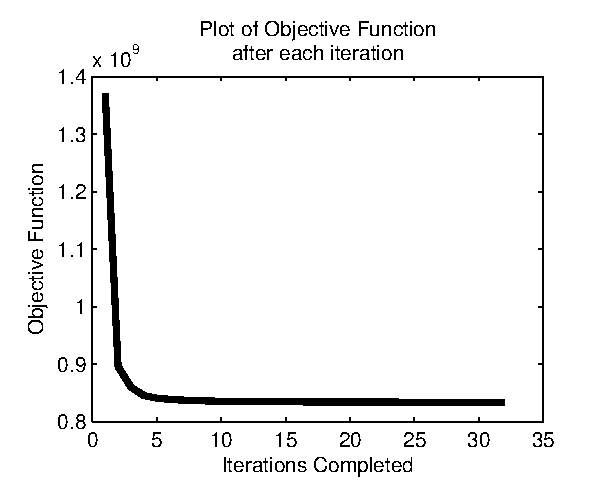
\includegraphics[width=0.46\textwidth]{4.2.eps}
\end{center}
\label{fig:4.2}
\end{figure}

\item As shown in Figure~\ref{fig:4.3}, the objective function still decreases
monotonically with each iteration. However, the objective function achieves a
lower value, although the number of iterations required to converge increases.
\begin{figure}[h]
\caption{Objective function after each iteration, for $K = 10$ and $K = 16$}
\begin{center}
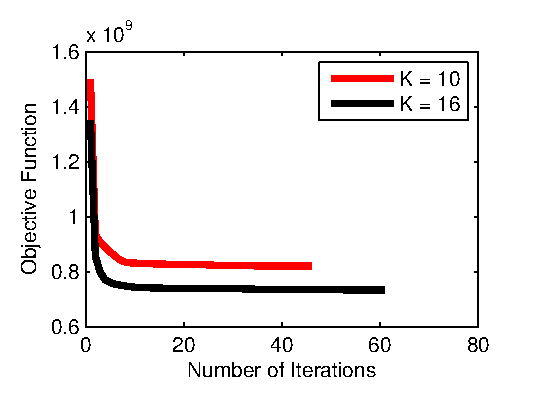
\includegraphics[width=0.46\textwidth]{4.3.eps}
\end{center}
\label{fig:4.3}
\end{figure}

\item The results are given in Table~\ref{tab:4.4}. \\

\begin{table}
\centering
\begin{tabular}{|c|c|c|}
\hline
Number of Clusters  & K-Means Accuracy  & Objective Function ($\times 10^9$)    \\
\hline
1                   & 11.40\%           & 2.8545                                \\
\hline
5                   & 44.84\%           & 0.9550                                \\
\hline
10                  & 59.68\%           & 0.8215                                \\
\hline
16                  & 67.57\%           & 0.7381                                \\
\hline
20                  & 71.26\%           & 0.6988                                \\
\hline
\end{tabular}
\caption{Data for Section 4, Part 4.}
\label{tab:4.4}
\end{table}

\item Although increasing the number of clusters would increase classification
accuracy and reduce the objective function, since we know in this case a
priori that there are $10$ classes of data points, it would probably be best
to use 10 clusters.
\end{enumerate}

\newpage
{\bf Code}

The following is the code used to implement K-means for Section 4 of the
assignment:

\small
\begin{verbatim}
% Inputs:
% X is 2D matrix, in which rows are data points and columns are features
%
% K is the number of clusters to be used
% 
% Outputs:
% clusters is a column vector in which each row is the cluster index of the
%     corresponding data point in X
%
% means is a K by num_features matrix containing the mean of each cluster
%
% num_iters is the number of iterations before convergence
%
% obj_func is the value of the objective function (defined in part 2) after
% each iteration

function [clusters means num_iters obj_func] = k_means(X, K)

  [num_points num_features] = size(X);

  % randomly choose K data points to be the initial cluster centers
  init_points = randsample(num_points, K);
  means = X(init_points, :);

  old_clusters = zeros(num_points,1);
  clusters = ones(num_points,1);

  num_iters = 0;

  while(any(clusters ~= old_clusters))
    num_iters = num_iters + 1;
    old_clusters = clusters;

    % reassign each data point to the cluster with the closest mean
    [clusters dists] = knnsearch(means, X);

    obj_func(num_iters) = sum(dists.^2);

    % recompute the mean of each cluster
    for i=1:K
      means(i,:) = mean(X(clusters &=&  i, :), 1);
    end
  end
end
\end{verbatim}
\normalsize

The following code was used to compute the classification accuracy of the
above K-means implementation, as well as to run multiple trials:

\small
\begin{verbatim}
% Inputs:
% X is 2D matrix, in which rows are data points and columns are features
%
% Y is vector of labels for each row of X
%
% K is a vector of numbers of clusters to be used (k_means is called trials
%   times for each value in K)
% 
% Outputs:
% acc is the fraction of correctly classified data points, averaged over
%   trials trials (acc is a vector, with one entry for each value of K)
%
function [acc obj_funs] = k_means_accuracy(X, Y, K, trials)

  acc = zeros(length(K),trials);
  obj_funs = zeros(length(K),trials);

  for k = 1:length(K)
    for trial = 1:trials

      [clusters, ~, ~, obj_fun] = k_means(X, K(k));

      num_correct = 0;

      % classify each cluster
      for cluster = 1:K(k)
        guess = mode(Y(clusters &=&  cluster));
        num_correct = num_correct + sum(guess &=&  Y(clusters &=&  cluster));
      end

      acc(k, trial) = num_correct ./ length(Y);
      obj_funs(k, trial) = obj_fun(end);
    end
  end

  % average over trials
  acc = mean(acc, 2);
  obj_funs = mean(obj_funs, 2);

end
\end{verbatim}
\end{document}
